\documentclass[12pt]{exam}
\usepackage[utf8]{inputenc}

\usepackage[margin=1in]{geometry}
\usepackage{amsmath,amssymb}
\usepackage{multicol}
\usepackage{hyperref}
\usepackage{graphicx}
\usepackage{color}
\usepackage{listings}
\usepackage{xcolor} 

\definecolor{darkgreen}{RGB}{0,100,0}

\lstset{
    language=Python,
    basicstyle=\ttfamily,
    keywordstyle=\color{blue},
    commentstyle=\color{gray},
    stringstyle=\color{darkgreen},
    breaklines=true
}

\newcommand{\class}{CS 5060}
\newcommand{\term}{Fall 2024}
\newcommand{\examnum}{Midterm Exam}
\newcommand{\examdate}{10/10/2024}
\newcommand{\timelimit}{10/14/2024 By End of Day}


\pagestyle{head}
\firstpageheader{}{}{}
\runningheader{\class}{\examnum\ - Page \thepage\ of \numpages}{\examdate}
\runningheadrule


\begin{document}

\noindent
\begin{tabular*}{\textwidth}{l @{\extracolsep{\fill}} r @{\extracolsep{6pt}} l}
\textbf{\class} & \textbf{Name: Nate Stott} \\
\textbf{\term} &&\\
\textbf{\examnum} &&\\
\textbf{\examdate} &&\\
\textbf{Time Limit: \timelimit}
\end{tabular*}\\
\rule[2ex]{\textwidth}{2pt}

This exam contains \numpages\ pages (including this cover page) and \numquestions\ questions.\\
The total of points is \numpoints.

This test is open notes but not open-neighbor.  Please read each question carefully before deciding on an answer.  A clear and concise statement or paragraph is much better than long answers with no focus on short written responses to these questions. 

I have taken the liberty of organizing this as I would an assignment rather than a classical exam. I hope that you take the time to learn and understand this. I imagine this will be a moderately pleasant venture if you do so.

Mario Mercy Option: As long as you get 3 of these questions with 75\%, the overall exam score will be at least 75\%.



\begin{center}
Grade Table \\
\addpoints
\gradetable[v][questions]
\end{center}

\noindent
\rule[2ex]{\textwidth}{2pt}

\begin{questions}


\question[20] Question 1: Algorithm Pseudocode (40 points)
\addpoints

Write pseudocode to describe the following four algorithms:\\

\begin{itemize}
    \item \textbf{Optimal Stopping Problem}: Describe the process of stopping optimally to maximize the expected reward.\\

    In the classic secretary problem, you interview candidates one by one and must decide immediately whether to hire each one. The optimal strategy involves two phases: first, reject the initial 37\% of candidates (approximately  $n/e$, where $n$ is the total number). This phase allows you to gather information. Afterward, hire the first candidate who is better than all those you’ve seen. \\

    This strategy gives you about a 37\% chance of selecting the best candidate over many trials. However, the primary goal of the algorithm isn’t necessarily to find the absolute best candidate, but rather to identify a "good enough" candidate who can start soon. While the approach doesn't guarantee success, it maximizes the likelihood of making a satisfactory choice given the constraints. The main challenge lies in balancing immediate rewards with potential future options, ensuring that hiring occurs in a timely manner while still aiming for a candidate who meets or exceeds the established standard. \\

    \begin{lstlisting}
import math

def secretary_problem(candidates):
    n = len(candidates)
    # Reject the first 37% of candidates
    threshold = math.floor(n / math.e)

    # Phase 1: Reject the first 37% of candidates
    # Find the best in the rejected candidates
    best_seen = max(candidates[:threshold])  

    # Phase 2: Hire the first candidate better than all seen so far
    for i in range(threshold, n):
        if candidates[i] > best_seen:
            hire(candidates[i])
            # End the process after hiring
            return  

    # If no candidate is better, then great we found the best!
    hire(best_seen)

def hire(candidate):
    print(f"Hired candidate: {candidate}")
    \end{lstlisting}
    
    \item \textbf{Multi-Armed Bandit Problem}: Write pseudocode for exploring and exploiting multiple options to maximize cumulative reward.\\

    For each round, the algorithm decides whether to explore (randomly select an arm) or exploit (choose the arm with the highest estimated reward) based on the epsilon value. If exploring, it picks a random arm; if exploiting, it selects the arm with the highest estimated value. After choosing an arm, it pulls that arm to get a reward, updates the counts and estimated values for that arm, and tracks the total reward earned across all rounds. The final output is the total reward collected, allowing evaluation of the strategy's performance. \\

    \begin{lstlisting}
def multi_armed_bandit(num_arms, epsilon, num_rounds):
    # Count of pulls for each arm
    counts = [0] * num_arms 
    # Estimated values for each arm
    values = [0.0] * num_arms 
    # Cumulative reward
    total_reward = 0 

    for _ in range(num_rounds):
        if random() < epsilon:
            # Explore with probability epsilon
            # Randomly choose an arm
            chosen_arm = random.randint(0, num_arms - 1) 
        else:
            # Exploit with probability 1 - epsilon
            # Choose the arm with the highest estimated value
            chosen_arm = values.index(max(values))  

        # Get the reward from the chosen arm
        reward = pull_arm(chosen_arm)   
        # Update counts for the chosen arm
        counts[chosen_arm] += 1
        # Update estimated value
        values[chosen_arm] += (reward - values[chosen_arm]) / counts[chosen_arm]  
        # Update cumulative reward
        total_reward += reward

    return total_reward
    \end{lstlisting}
    
    \item \textbf{Option Valuation}: Provide pseudocode for calculating the value of a financial option, considering potential future prices.\\

    In each simulation, it generates a random variable to model potential stock price movements based on a geometric Brownian motion formula, which accounts for the risk-free rate and volatility. The final stock price is computed, and the payoff of the option (the profit if the stock price exceeds the strike price) is determined. The total payoff across all simulations is averaged, and this average is discounted back to present value to find the option's value. This method helps in estimating how much the option is worth based on the likelihood of future stock price movements. \\

    \begin{lstlisting}
import numpy as np
import math

def european_option_valuation(initial_price, strike_price, 
risk_free_rate, volatility, time_to_maturity, num_simulations):
    total_payoff = 0

    for _ in range(num_simulations):
        # Generate a random normal variable for the simulation
        random_normal = np.random.normal()
        
        # Calculate the final stock price using the GBM formula
        final_price = initial_price * math.exp(
            (risk_free_rate - 0.5 * volatility ** 2) * time_to_maturity + 
            volatility * random_normal * math.sqrt(time_to_maturity)
        )

        # Calculate the call option payoff
        payoff = max(final_price - strike_price, 0)
        total_payoff += payoff

    # Calculate the average payoff and discount it to present value
    average_payoff = total_payoff / num_simulations
    option_value = average_payoff * math.exp(-risk_free_rate * time_to_maturity)

    return option_value
    \end{lstlisting}
    
    \item \textbf{Insurance Algorithm}: Detail the pseudocode for pricing an insurance product based on probabilistic risk models.\\

    The code simulates the pricing of an insurance product using Monte Carlo methods. It takes inputs like expected claims, operating costs, a risk factor, the number of simulations, and a profit margin. For each simulation, it randomly determines if a claim occurs based on the risk factor and generates claim severity using an exponential distribution. It then calculates the average claims, adds operating costs to find the total premium, and applies the profit margin to arrive at the final price of the insurance product. This approach helps insurers estimate a competitive and viable price based on probabilistic claims data. \\

    The final\_price in the code represents the price of the insurance product as a whole, which could be intended for a pool of policyholders rather than just an individual. However, it can be adapted for an individual by adjusting how claims, operating costs, and risk factors are defined based on individual circumstances. \\

    \begin{lstlisting}
import numpy as np

def price_insurance_product(operating_costs, 
risk_factor, num_simulations, profit_margin):
    # Step 1: Initialize variables
    total_claims = 0

    # Step 2: Simulate claims based on probabilistic risk models
    for _ in range(num_simulations):
        # Generate random variables for claim occurrence and severity
        claim_occurrence = _generate_claim_occurrence(risk_factor)
        claim_severity = _generate_claim_severity()

        # Calculate total claims for this simulation
        total_claims += claim_occurrence * claim_severity

    # Step 3: Calculate average claims from simulations
    average_claims = total_claims / num_simulations

    # Step 4: Calculate total premium
    total_premium = average_claims + operating_costs

    # Step 5: Calculate final price based on profit margin
    final_price = total_premium * (1 + profit_margin)

    return final_price

def _generate_claim_occurrence(risk_factor):
    # Generate a random value to determine if a claim occurs
    # Uniform distribution between 0 and 1
    random_value = np.random.uniform(0, 1)  
    # Claim occurs or not
    return 1 if random_value < risk_factor else 0  

def _generate_claim_severity():
    # Generate a random value for claim severity based on a predefined distribution
    # Example: claims severity follows an exponential distribution
    return np.random.exponential()  
    \end{lstlisting}

    
\end{itemize}

\textit{Each pseudocode description should include input, output, and a high-level explanation of key steps.}



\question[40] Question 2: Impact of Randomness on Algorithms (30 points)

Consider how randomness affects each of the algorithms discussed in Question 1. For each algorithm, explain how the behavior changes when using different random distributions (uniform, normal, and beta with skew).

\begin{itemize}
    \item How would the \textbf{Optimal Stop} algorithm change with these distributions?\\

    \textbf{uniform distribution}: the classic strategy of rejecting the first 37\% of candidates remains effective, giving about a 37\% chance of selecting the best candidate. \\
    
    \textbf{normal distribution}: the performance can vary based on the mean and standard deviation; a low standard deviation may make it harder to identify standout candidates, while a high standard deviation could enhance the chances of finding an exceptional one, possibly necessitating a more tailored threshold. \\
    
    \textbf{skewed beta distribution}: the strategy's effectiveness further depends on the direction of the skew. A right-skewed distribution may yield few competitive candidates during the rejection phase, while a left-skewed one could present more high-value candidates. In such cases, adjusting the threshold or employing a more adaptive approach may be necessary to maximize hiring chances. \\

    \textbf{bimodal distribution}: with a bimodal distribution, the presence of two distinct peaks suggests that there may be two groups of candidates with different qualifications or attributes. This could complicate the classic strategy, as the algorithm might need to recognize which mode represents higher-quality candidates. An adaptive approach could be beneficial, where the rejection threshold is adjusted based on the observed candidates’ qualities, allowing for better identification of which mode to prioritize. Consequently, this might lead to improved chances of selecting the best candidate among the two groups. \\
    

    \item How does the \textbf{Multi-Armed Bandit} algorithm's decision-making change?\\

    
    \textbf{uniform distribution}: rewards are predictable and consistent, allowing the algorithm to explore effectively and quickly identify the highest-value arm. This leads to balanced performance and steady total rewards across rounds. \\
    
    \textbf{normal distribution}: the impact depends on the mean and variance. Low variance facilitates rapid identification of the best arm, while high variance can introduce uncertainty, potentially resulting in suboptimal exploitation if the algorithm overly favors a volatile arm.\\
    
    \textbf{skewed beta distribution}: the decision-making process becomes more complex. A right-skewed distribution may slow the identification of higher-value arms, whereas a left-skewed distribution could lead to quick exploitation but risks overconfidence in a particular arm. \\

    \textbf{bimodal distribution}: with a bimodal distribution, the presence of two peaks in the reward structure indicates that there are two distinct groups of arms, each with different expected rewards. This can complicate the decision-making process, as the algorithm must discern which mode offers better long-term rewards. The challenge lies in balancing exploration between both peaks to identify the optimal arm while avoiding overcommitment to one that may appear initially promising. An adaptive strategy might be needed to adjust exploration rates dynamically, enabling the algorithm to effectively switch focus between the two modes based on observed rewards. \\
    
    \item How does the randomness impact the \textbf{Option Valuation} algorithm?\\
    
    \textbf{uniform distribution}: may lead to oversimplified estimations that fail to reflect the complexities of financial markets, resulting in potentially inaccurate option valuations. \\
    
    \textbf{normal distribution}: aligns better with the assumptions of geometric Brownian motion, providing a more realistic simulation of stock prices. However, it may still underestimate extreme movements, leading to conservative valuations. \\
    
    \textbf{skewed beta distribution}: allows for greater flexibility in modeling stock price behavior, capturing various market conditions more accurately. This approach can yield more precise option valuations by reflecting the potential for both high and low price movements based on the chosen skew. \\

    \textbf{bimodal distribution}: in scenarios where stock price movements exhibit a bimodal distribution, the presence of two distinct peaks may indicate that stock prices can cluster around two different levels due to varying market conditions or investor behaviors. This can complicate option valuations, as the algorithm must account for the likelihood of significant price shifts between these two modes. Consequently, the algorithm may need to adjust its simulations to ensure that both potential outcomes are adequately represented, which can lead to more accurate option pricing but may also increase computational complexity. Understanding the implications of bimodal distributions is vital for capturing the true value of options in such markets. \\
    
    \item How would randomness alter the performance of the \textbf{Insurance Algorithm}?\\
    
    \textbf{uniform distribution}: may oversimplify risk assessments, leading to inaccurate estimations of claim occurrences and potentially resulting in insurance premiums that are either too low, exposing the insurer to losses, or too high, making the product uncompetitive. \\
    
    \textbf{normal distribution}: allows for clustering around a mean value, providing a more nuanced perspective on risk. However, if not parameterized correctly, it could underestimate potential losses or overly inflate prices, impacting competitiveness. \\

    \textbf{skewed beta distribution}: offers even greater flexibility, accurately capturing the complexities of real-world claims, particularly when certain outcomes are more likely than others. This approach enables more realistic estimations of average claims, leading to more appropriate pricing strategies. However, accurately estimating the distribution parameters is critical, as misestimations can still yield flawed premium calculations. \\

    \textbf{bimodal distribution}: when claims are modeled using a bimodal distribution, the presence of two distinct peaks suggests that there may be two different groups of claims with varying severities or occurrences. This can complicate the pricing strategy, as the algorithm must account for the likelihood of significant claims from both modes. The challenge lies in effectively balancing the premiums to reflect the potential risks from each group. If not handled correctly, this could lead to underpricing for one group while overpricing for another, ultimately affecting the competitiveness and profitability of the insurance product. Understanding how to manage and adapt to a bimodal distribution is crucial for accurate risk assessment and premium determination. \\

    
\end{itemize}

Additionally, consider the following example of an interesting distribution (shown in Figure \ref{fig:distribution}), and describe how you think it might impact these algorithms. Draw any connections between the shape of the distribution and potential algorithm behavior.


\begin{figure}[htbp] 
    \centering
    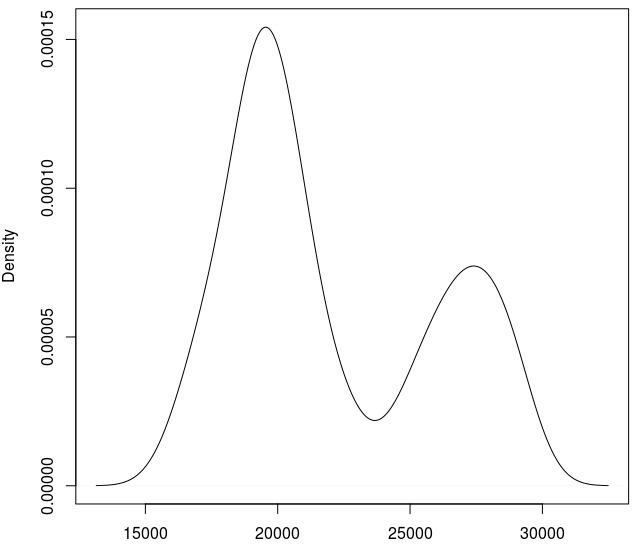
\includegraphics[width=0.75\linewidth]{interesting_distribution.png}
    \caption{A distribution that is fairly common in a certain type of field we have discussed at some length in our course lectures.}
    \label{fig:distribution}
\end{figure}



\question[20] Question 3: Nature of the Algorithms (20 points)

Discuss the following properties of the algorithms:

\begin{enumerate}
    \item \textbf{Topology in the Optimal Stop Algorithm}: How does the state-space or topology of decisions evolve? How does this affect finding the optimal stopping point?\\

    The state-space in the Optimal Stop Algorithm, particularly in the secretary problem, can be visualized as a binary tree. Each decision point branches into two outcomes: Reject and Accept. Initially, the algorithm starts at the root with the first candidate. Choosing to Reject extends the tree, while Accepting terminates that branch, indicating the candidate has been Hired. \\

    As candidates are rejected, the tree grows deeper, reflecting the accumulation of information and the complexity of decisions. Each Reject adds a new layer, allowing for better-informed choices later, but also increasing the risk of missing an optimal candidate. This binary tree topology emphasizes the balance between exploration and exploitation, highlighting how strategic decisions shape the algorithm's effectiveness in identifying the best stopping point. \\
    
    \begin{lstlisting}
          Start
            |
        +---+---+
        |       |
     Reject     Accept
        |            |
     +--+--+        (Hired)
     |     |        
  Reject   Accept   
     |          |
  +--+--+      (Hired)
  |     |       
Reject  Accept  
   |         | 
   .       (Hired)
   .    
    \end{lstlisting}

    
    \item \textbf{Explore/Exploit Trade-offs in Multi-Armed Bandits}: How do different strategies (epsilon-greedy, Thompson sampling) handle the explore/exploit trade-off in various conditions?\\
    
    The \textbf{epsilon-greedy strategy} allocates a fixed probability \( \epsilon \) for exploration and \( 1 - \epsilon \) for exploitation. While straightforward and effective in stationary environments, this method can lead to inefficiencies in non-stationary contexts, as the fixed exploration rate may result in unnecessary exploration of suboptimal arms or missed opportunities for high rewards.\\
    
    On the other hand, \textbf{Thompson Sampling} utilizes a Bayesian framework, maintaining probabilistic models of expected rewards for each arm. By sampling from these distributions, it adapts its strategy based on uncertainty, exploring more when estimates are uncertain and exploiting when confidence is high. This flexibility makes it particularly effective in dynamic environments where reward distributions can change. However, it is also more computationally intensive.\\
    
    \item \textbf{Option Valuation Model}: How do assumptions (e.g., volatility, time) change the option valuation model? What might happen under extreme assumptions?\\

    The assumptions in an option valuation model—\textbf{initial price}, \textbf{strike price}, \textbf{risk-free rate}, \textbf{volatility}, \textbf{time to maturity}, and \textbf{number of simulations}—significantly influence the valuation outcome. Here's how each assumption affects the model and the potential consequences of extreme assumptions: \\

    \textbf{Initial Price}: serves as the foundation for the valuation model. Changes in the initial price directly affect future price projections and, consequently, the option's value. Underestimating the initial price can lead to a lower valuation, while overestimating it can inflate the option's worth. Extreme assumptions about the initial price can result in unrealistic valuations that don’t reflect current market conditions.\\

    \textbf{Strike Price}: determines the profitability of exercising the option. Changes in the strike price relative to the initial price alter the likelihood of the option being in-the-money. Setting an excessively high strike price may lead to a significant drop in the option’s value, while an unusually low strike price could inflate the value unrealistically. Extreme assumptions can create scenarios that don’t align with market realities.\\

    
    \textbf{Risk-Free Rate}: critical for discounting future payoffs. A higher risk-free rate decreases the present value of those payoffs, while a lower rate increases it. Extreme assumptions—such as setting the rate much higher or lower than market averages—can distort valuations significantly, leading to either overly pessimistic or optimistic pricing of options.\\

    \textbf{Volatility}: measures the expected price variation of the underlying asset. Higher volatility increases the chance of finishing in-the-money, enhancing the option’s value. However, assuming extreme volatility (either too high or too low) can lead to inflated or conservative valuations. For instance, excessive volatility might suggest an unrealistic level of risk and reward, while very low volatility could fail to capture potential market movements.\\

    \textbf{Time to Maturity}: influences how much value an option retains. A longer duration generally increases an option’s value due to more opportunities for favorable price changes. Extreme assumptions, such as very short or excessively long durations, can lead to unrealistic valuations. A very short time frame may undervalue the option, while a long time frame could suggest unreasonably high future profit potential.\\

    \textbf{Number of Simulations}: impacts the reliability of the valuation. A higher number of simulations can provide a more accurate reflection of potential price paths, capturing a broader range of outcomes. However, if too few simulations are used, the model may not adequately account for market variability, leading to unreliable valuations. Extreme assumptions about the number of simulations could oversimplify market dynamics or create unnecessary computational burdens without improving accuracy.\\
    
    \item \textbf{Effective Insurance Product Design}: What considerations improve the design of an insurance product? How does uncertainty and risk modeling influence pricing?\\

    Grouping individuals into a risk pool is fundamental to insurance, as it allows insurers to spread potential losses across a larger number of policyholders, thereby mitigating overall risk. This collective approach stabilizes premiums, making insurance products more sustainable and predictable. By aggregating risks, insurers can better estimate expected losses and set premiums accordingly, creating a more stable financial model.\\

    However, customization is crucial for maintaining customer satisfaction. While a standardized approach works for pooling risk, individual circumstances—such as specific risk factors or unique needs—require tailored coverage options. Offering personalized insurance solutions helps customers feel valued and understood, enhancing their overall experience. Balancing collective risk management with individual customization is key to developing effective insurance products that meet both financial and customer needs.\\

    The risk factor quantifies the likelihood of claims, but uncertainty regarding the distribution of those claims—whether normal, exponential, or bimodal—significantly impacts pricing strategies. Different distributions affect the expected loss calculations and risk premium adjustments. For instance, a normal distribution may yield predictable average losses, while a bimodal distribution suggests two distinct risk profiles that necessitate more complex pricing. If insurers misestimate the distribution, they risk either underpricing, leading to inadequate reserves, or overpricing, which could harm competitiveness.\\

    Moreover, volatility in claims associated with varying distributions can prompt higher premiums to buffer against unexpected high losses. Insurers must also consider regulatory requirements, as inaccurate distribution assumptions can lead to non-compliance and financial instability. Therefore, robust risk modeling and continuous reassessment of claims distributions are essential for developing accurate and competitive insurance pricing.\\
    
    
\end{enumerate}

\question[40] Insurance: Value of Subdivision
\addpoints

We are going to look at a simple insurance dataset (in the Canvas midterm module, a data file is provided named insurance.csv) where we only consider a few factors for 10,000 people: 

\begin{itemize}
    \item age (INT age of claimant)
    \item sex (BINARY As identified by the claimant)
    \item bmi (FLOAT bmi of claimant, NA if not claimant that year)
    \item children (INT children count per claimant, NA if not claimant that year)
    \item smoker (BINARY smoking status of claimant, NA if not claimant that year)
    \item region (STRING claimant regional ID, NA if not claimant that year)
\end{itemize}

PART 1 - Calculate the basic insurance rate for this population if we are looking at zero deductible policies and we need an 11 \% profit margin. What is the standard deviation and volatility of this portfolio?\\

Basic Insurance Rate: \$1970.90 \\

This is the average premium that individuals in the population would need to pay for their insurance coverage, including an 11\% profit margin. It reflects the expected claims cost spread across the entire insured population, including both claimants and non-claimants. \\

Standard Deviation of Claims: \$12110.01\\

This value indicates the variability or dispersion of the claims amounts from the average claim. A high standard deviation means that there is a wide range of claim amounts—some individuals may have very high claims while others have low claims. In this case, the significant standard deviation suggests that while some claims are relatively low, there are also some very large claims, which can impact overall insurance costs and risk.\\

Volatility of the Portfolio: 0.91\\

Volatility measures the relative risk of the insurance portfolio. It's calculated as the standard deviation of claims divided by the mean claims amount. A volatility of 0.91 means that the standard deviation is nearly equal to the average claim amount, indicating high relative risk. This suggests that the potential for large claims is significant compared to the average claim, and it may signal a need for the insurer to manage risk carefully.\\

PART 2 - Calculate the tiered insurance rate (with the same 11\% profit margin) for this population by breaking up the insurance product by age categories of [18-22, 23-30, 31-48, and 49+]. What is the standard deviation and volatility of this portfolio?\\

Age Category: 18-22\\
Tiered Insurance Rate: \$1250.77\\
Standard Deviation of Claims: \$11487.28\\
Volatility: 1.37\\

Age Category: 23-30\\
Tiered Insurance Rate: \$1543.10\\
Standard Deviation of Claims: \$11543.58\\
Volatility: 1.11\\

Age Category: 31-48\\
Tiered Insurance Rate: \$1963.76\\
Standard Deviation of Claims: \$11952.85\\
Volatility: 0.91\\

Age Category: 49+\\
Tiered Insurance Rate: \$2591.06\\
Standard Deviation of Claims: \$11468.97\\
Volatility: 0.65\\

The analysis provides insights into insurance rates segmented by age categories, with a basic insurance rate of \$1970.90 for the overall population. The tiered rates reveal that younger individuals (ages 18-22 and 23-30) have lower rates (\$1250.77 and \$1543.10), indicating fewer or less costly claims but higher volatility, suggesting significant variation in claims among those who do file.\\

In contrast, older age groups (31-48 and 49+) show higher tiered rates (\$1963.76 and \$2591.06), reflecting the typical trend of increased healthcare costs with age. The findings highlight the importance of considering both claimants and non-claimants in risk assessments, as well as the variability of claims within age groups, which is crucial for setting accurate insurance rates.\\

PART 3 - Calculate the same in PART 2, but add sex to the calculation. Compare just using the sex parameter as compared to both age and sex. \\

Age Category: 18-22, Sex: female\\
Tiered Insurance Rate: \$1072.87\\
Standard Deviation of Claims: \$10141.35\\
Volatility: 1.34\\

Age Category: 18-22, Sex: male\\
Tiered Insurance Rate: \$1431.71\\
Standard Deviation of Claims: \$12593.16\\
Volatility: 1.38\\

Age Category: 23-30, Sex: female\\
Tiered Insurance Rate: \$1443.16\\
Standard Deviation of Claims: \$10029.66\\
Volatility: 1.04\\

Age Category: 23-30, Sex: male\\
Tiered Insurance Rate: \$1635.86\\
Standard Deviation of Claims: \$12815.42\\
Volatility: 1.15\\

Age Category: 31-48, Sex: female\\
Tiered Insurance Rate: \$1841.52\\
Standard Deviation of Claims: \$11410.16\\
Volatility: 0.92\\

Age Category: 31-48, Sex: male\\
Tiered Insurance Rate: \$2085.39\\
Standard Deviation of Claims: \$12442.06\\
Volatility: 0.89\\

Age Category: 49+, Sex: female\\
Tiered Insurance Rate: \$2541.61\\
Standard Deviation of Claims: \$10284.44\\
Volatility: 0.61\\

Age Category: 49+, Sex: male\\
Tiered Insurance Rate: \$2639.35\\
Standard Deviation of Claims: \$12547.32\\
Volatility: 0.69\\

The data indicates a clear relationship between age, sex, and tiered insurance rates, with older individuals generally facing higher rates. For instance, the 49+ age group shows significantly elevated rates (\$2541.61 for females and \$2639.35 for males) compared to younger categories. Additionally, males tend to have higher insurance rates than females across all age groups, suggesting that male claimants may incur greater average claims.\\

The variability in claims, as reflected by the standard deviations, is notably high for younger age groups, indicating that while their average rates are lower, the potential for large claims is substantial. In contrast, older age groups display lower volatility, suggesting more predictable healthcare needs. These insights underscore the importance of tailoring insurance products to account for these demographic factors, allowing insurers to manage risk effectively while providing suitable coverage.\\

------

Sex: female\\
Tiered Insurance Rate: \$1864.80\\
Standard Deviation of Claims: \$11128.70\\
Volatility: 0.89\\

Sex: male\\
Tiered Insurance Rate: \$2075.01\\
Standard Deviation of Claims: \$12971.03\\
Volatility: 0.93\\

The data shows that males have a higher tiered insurance rate of \$2075.01 compared to \$1864.80 for females, indicating greater average claims costs. Both genders exhibit significant variability in claims, with standard deviations of \$11,128.70 for females and \$12,971.03 for males. Males also show slightly higher volatility at 0.93 versus 0.89 for females. These findings highlight the importance of considering gender differences in insurance pricing strategies.\\

PART 4 - Comment on the change in risk for the portfolio and the anticipated benefits from subdividing the insurance product. Calculate what the prices would be if you could break the product into known claimants (ie: you know which people will be claimants and who will not be this year). What does the cost rise to for the annual rate on the claimants? \\

Insurance Rate for Known Claimants: \$14730.17\\
Standard Deviation of Claims (Known Claimants): \$12110.01\\
Volatility (Known Claimants): 0.91\\

Focusing on known claimants raises the insurance rate to \$14,730.17, reflecting the concentrated risk of insuring only those expected to file claims. The standard deviation of \$12,110.01 indicates high variability in claims costs, while a volatility of 0.91 shows considerable uncertainty among these individuals.\\

This subdivision allows for more accurate pricing and risk assessment, enabling insurers to tailor rates based on specific claimant profiles. However, it also increases risk concentration, making the insurer more dependent on the claims behavior of a smaller group. While it enhances precision in risk management, the elevated rate highlights the financial implications of insuring higher-risk individuals.\\

\end{questions}


\end{document}
